\documentclass{article}
\usepackage[utf8]{inputenc}
\usepackage[english]{babel}
\usepackage{amsmath}
\usepackage{amssymb}
\usepackage{setspace}
\usepackage{natbib} 
\usepackage{graphicx}
\usepackage{subfig}
\usepackage{comment}
\usepackage[backgroundcolor=pink,linecolor=red]{todonotes}
\usepackage{fullpage}
\usepackage[hidelinks]{hyperref}
\usepackage{xcolor}
\usepackage{comment}

\onehalfspacing


\title{Part 1 Demultiplexing | BIO 622}
\author{Jared Galloway}
\date{}                                           % Activate to display a given date or no date

\begin{document}
\maketitle

\section*{Part 1}

%\newpage
\begin{enumerate}
 \item 

\begin{center}
 \begin{tabular}{||c c||} 
 \hline
 Filename & Read \\ [0.5ex] 
 \hline\hline
 $1294_S1_L008_R1_001.fastq.gz$ & Read 1 \\ 
 \hline
 $1294_S1_L008_R2_001.fastq.gz$ & Index 1 \\
 \hline
 $1294_S1_L008_R3_001.fastq.gz$ & Index 2 \\
 \hline
 $1294_S1_L008_R4_001.fastq.gz$ & Read 2 \\
 \hline
\end{tabular}
\end{center}

\begin{description}

    \item

    \begin{figure}[h!!!!]
        \center{
        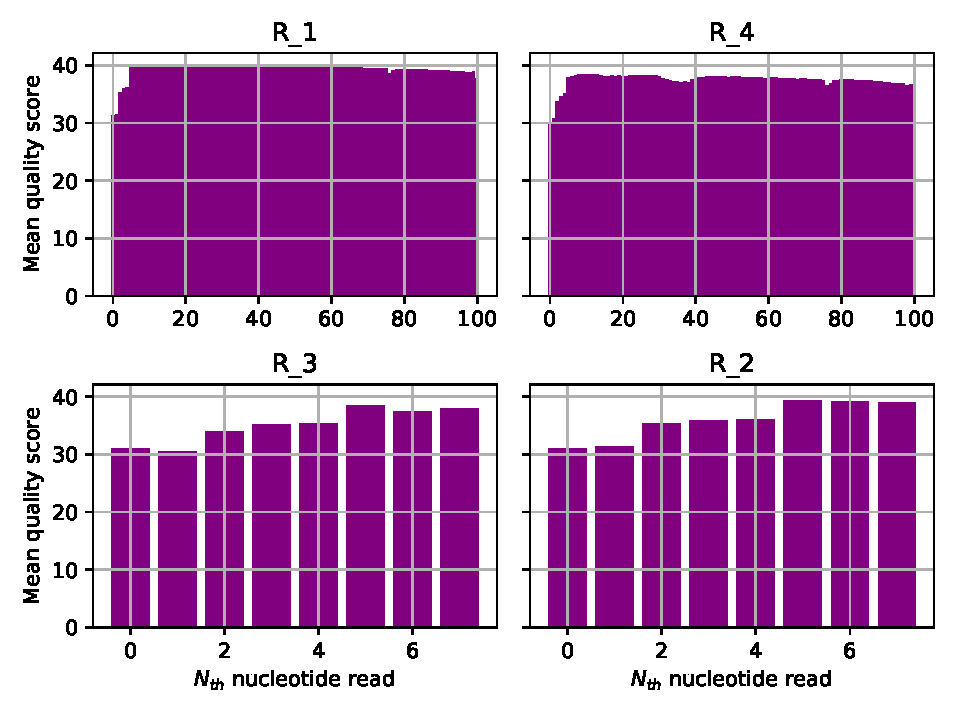
\includegraphics[width=0.8\textwidth]{../pos_dist_plots/position_mean_quality.pdf}
        }
        \caption{
        \label{fig:my-label1} Distribution of average quality score R1}
    \end{figure}

     \item

    Due to the first two biologcal reads -- for both R1 and R2 -- 
    are quite low $\approx < 36$, I would set the cutoff for 36, to make 
    sure we are getting high quality biolocial reads.

    \newpage
    \item

    To find the total number of N's within the two index reads, 
    I used the following bash command


    zcat emp\_files/1294\_S1\_L008\_R[2-3]* | awk 'NR\%4==2' | grep N | wc -l > countN\_Index.txt

\end{description}
\end{enumerate}

\section*{Part 2}

\textbf{Problem}: this problem is defined by seperating out reads on a flow cell based upon
the reported barcode. This means that both index reads from each pair must match and be high
quality in order to be succefully demultiplexed. 
If the Index pairs are 
\textit{valid} (meaning above the quality cutoff, and exist in pre-defined set of indices)  
yet they do match for both pairs of a given read, then we put them in a hopped fastq file.
for \textit{not valid} indices, we put the read in an undefined fastq file.

\textbf{Output}: For this, I'm going to make two output fastq files for each valid index 
for each one of the paired end reads. And two files for undefined and two files for hopped.

\textbf{Test Files}: I'm going to make four test files which have three respective reads 
in each, one for each of the catagories mentioned above. 

(bgmp\_py3) n221 13:30 [demultiplexing-jgallowa07] \$ ./P2.py -fq test\_files/R[1-4]* -fi emp\_files/indexes.txt 
Number of hopped reads = 1
Number of undefined reads = 1
Number of valid reads = 1

\textbf{Algorithm \& High-Level functions} : Found in psuedo\_code/ folder





 






\end{document}
